\documentclass{report}
\usepackage[spanish]{babel}
\usepackage[utf8]{inputenc}
\usepackage{graphicx, url, longtable, float, titlesec, hyperref, enumitem, verbatim, dingbat}
\usepackage[dvipsnames]{xcolor}
\usepackage[margin=4cm]{geometry}

\usepackage{enumitem,amssymb}
\newlist{todolist}{itemize}{2}
\setlist[todolist]{label=$\square$}
\usepackage{pifont}
\newcommand{\cmark}{\ding{51}}%
\newcommand{\xmark}{\ding{55}}%
\newcommand{\done}{\rlap{$\square$}{\raisebox{2pt}{\large\hspace{1pt}\cmark}}%
\hspace{-2.5pt}}
\newcommand{\wontfix}{\rlap{$\square$}{\large\hspace{1pt}\xmark}}

\title{Proyecto AS}
\author{Francisco Fernández Condado}
\date{November 2024}

\titleformat{\chapter}[display]
  {\normalfont\bfseries}{}{0pt}{\Huge}

\begin{document}
    \begin{titlepage}
        \centering
        
\includegraphics[width=0.7\linewidth]{img/bie.jpg}\\
        \vspace{3.5cm}
        \Huge Agenda cultural de Euskadi\\
        \vspace{2.5cm}
        \Large Administración de Sistemas\\
        \vspace{0.5cm}
        \large 4º Curso\\
        \vspace{3cm}
        \LARGE Grado en Ingeniería Informática de Gestión y Sistemas de Información\\
        \vspace{1cm}
        \large Francisco Fernández Condado\\
        \vspace{0.5cm}
        \large 24 de noviembre de 2024\\
    \end{titlepage}
    
    \tableofcontents
    \listoffigures
    \listoftables
    
    \chapter{Introducción}
        Este proyecto propone la creación de una aplicación web funcional basándose en los contenedores de Docker y, de forma opcional, realizar el despliegue equivalente de Kubernetes.

        En este caso, la idea es crear un portal web interactivo que permita consultar la Agenda Cultural de Euskadi con actualizaciones en tiempo real. Para ello, se ha hecho uso de la información proporcionada en el \href{https://opendata.euskadi.eus/catalogo/-/kulturklik-agenda-cultural/}{portal Open Data del Servicio web del Gobierno Vasco}, que provee diferentes formas de acceso a la información completa.

        Se ha elegido hacer uso de un servidor web basado en nginx, que se encargará de redirigir las peticiones a un servidor Flask. La información de los eventos queda registrada en una base de datos PostgreSQL y, mediante un entorno adicional basado en Python, se actualizan los datos de los eventos a partir de la \href{https://opendata.euskadi.eus/apis/-/apis-open-data/}{API de Open Data} para contar con actualizaciones en tiempo real. Además, se cuenta con un entorno adicional que permite exportar los detalles de los eventos a un formato PDF, siendo más cómodo para imprimir o compartir en caso de ser necesario.

        \begin{figure}[H]
            \centering
            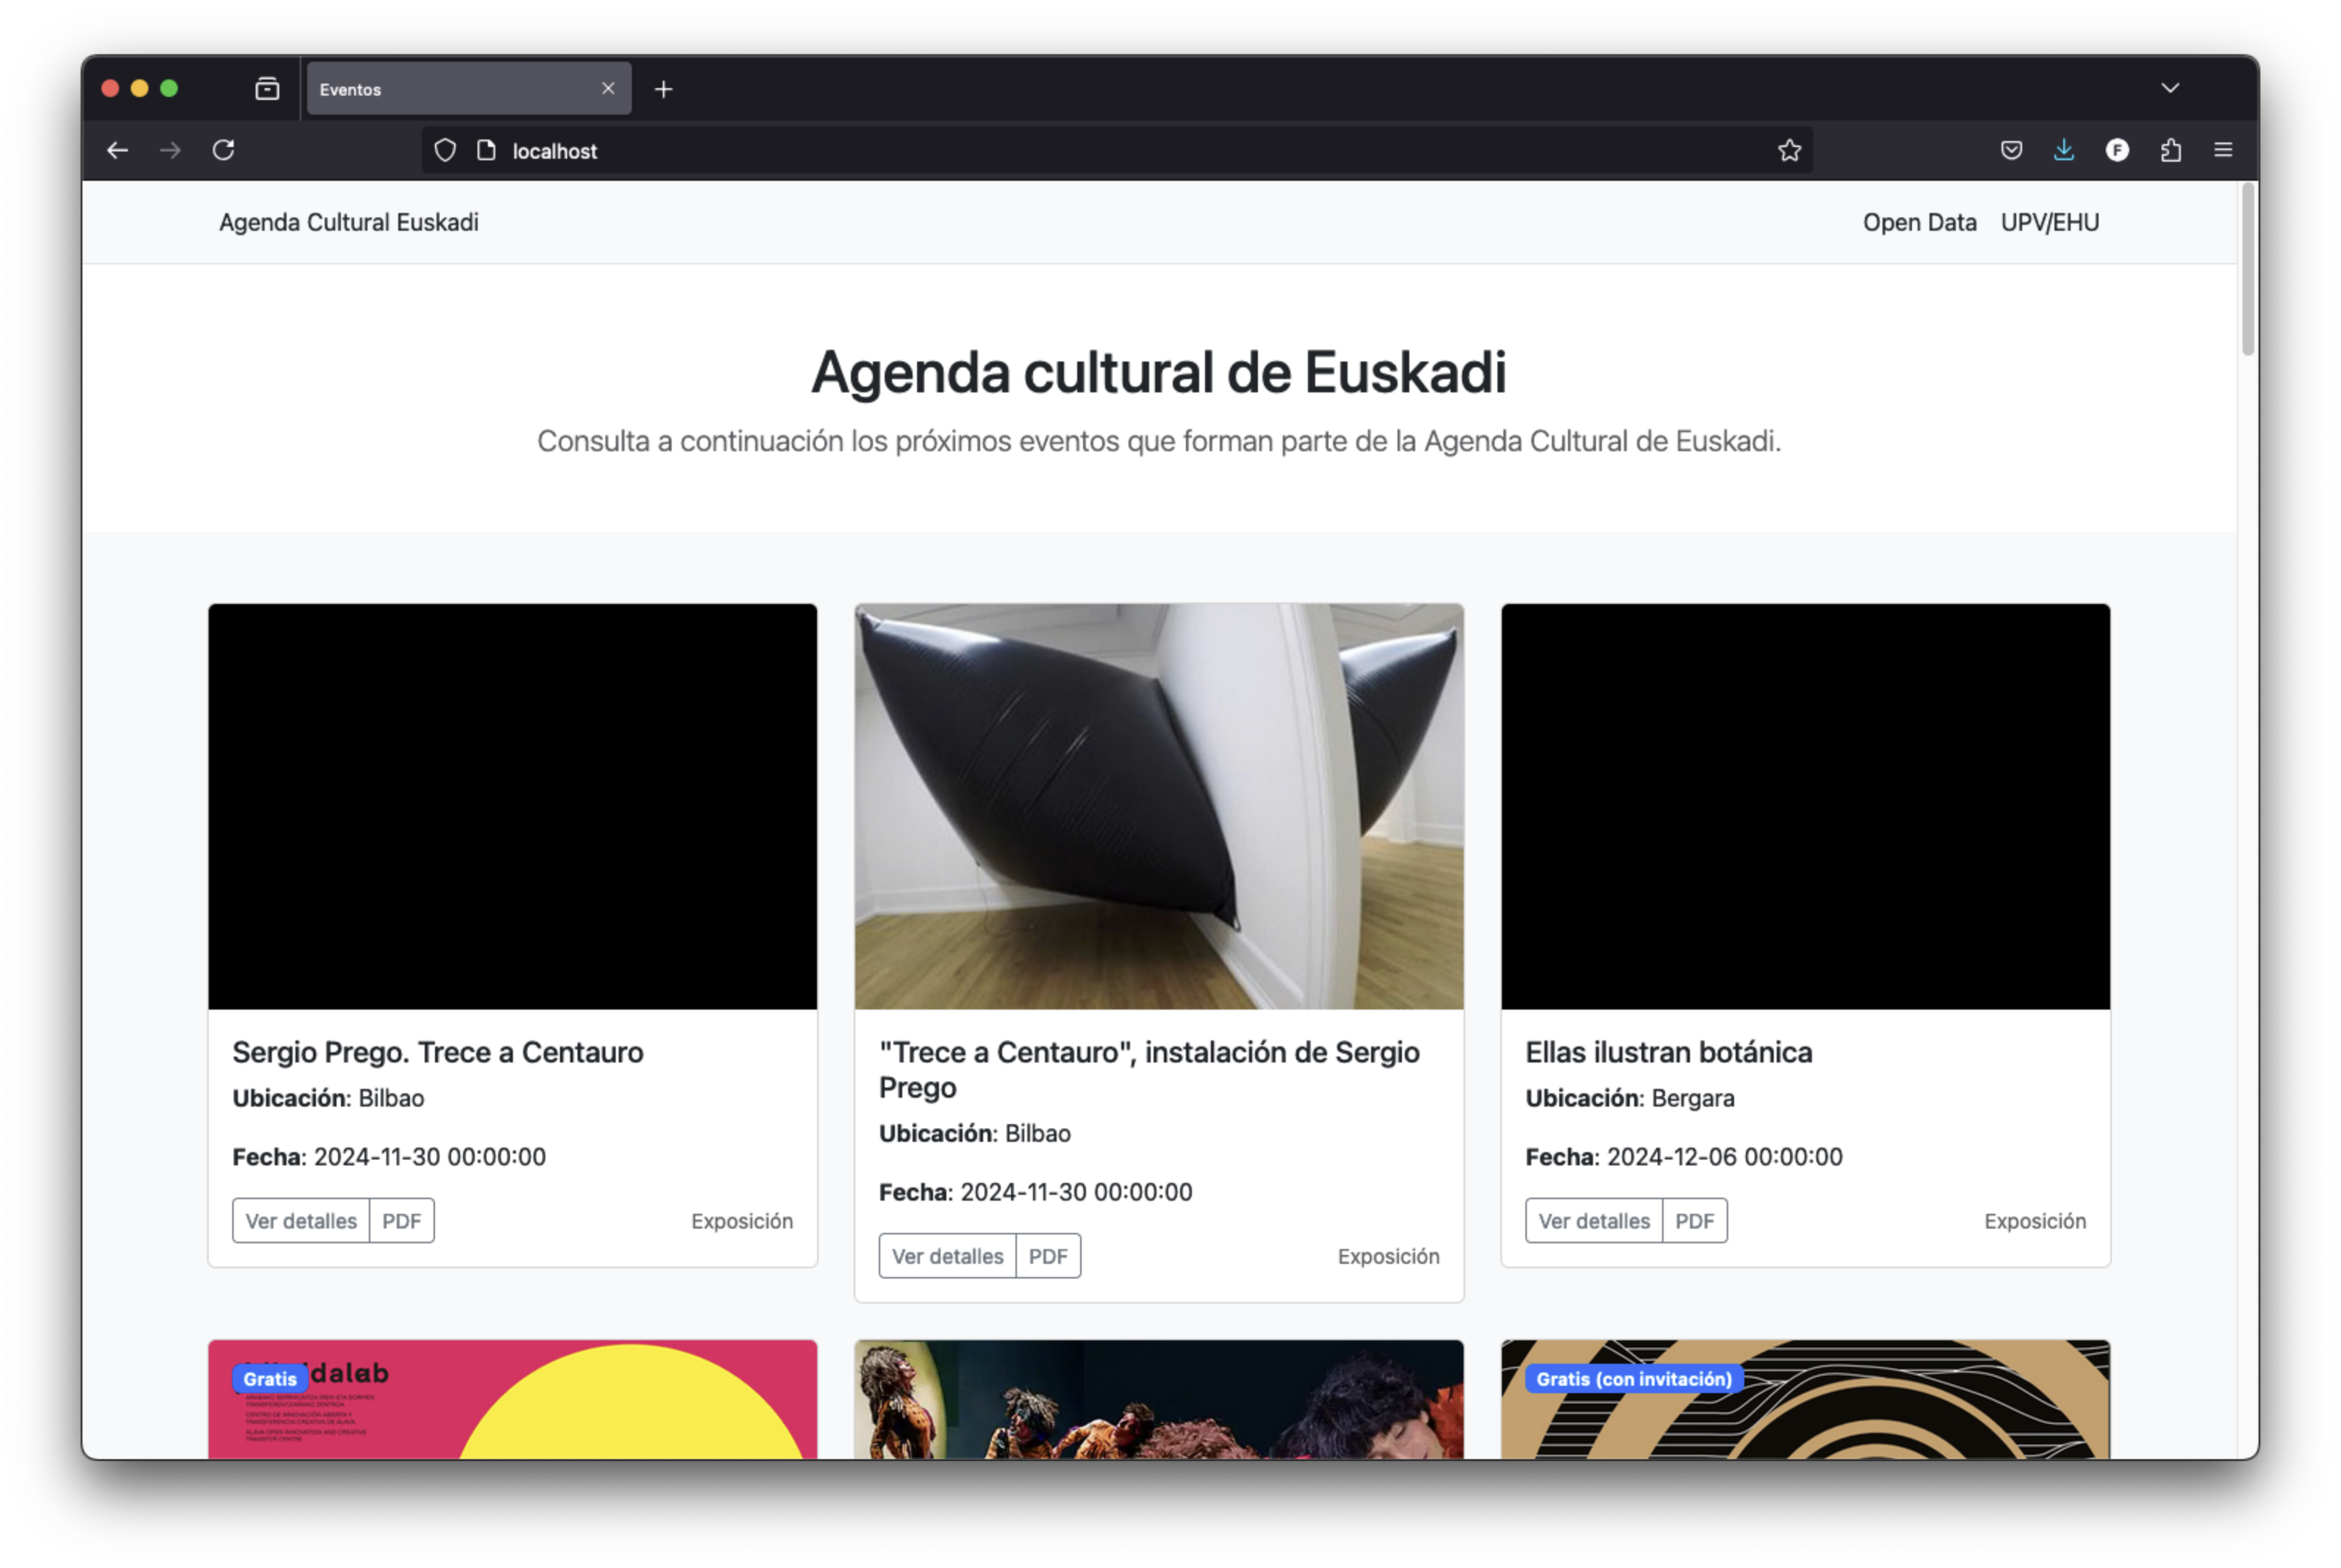
\includegraphics[width=0.8\linewidth]{img/general.png}
            \caption{Vista general de la aplicación}
            \label{fig:enter-label}
        \end{figure}

        De este modo, la aplicación web permite acceder a un catálogo actualizado en tiempo real de los eventos presentes en la Agenda Cultural de Euskadi, con un diseño sencillo basado en la librería \href{https://getbootstrap.com}{Bootstrap}. Accediendo al detalle completo, será posible consultar toda la información (fechas, descripción, coste, categoría, lugar de realización, enlaces adicionales, etc.), así como a un mapa que muestra la ubicación en la que se realizará el evento.

        El despliegue completo de la aplicación puede encontrarse en el siguiente repositorio de GitHub para su uso y descarga: \url{https://github.com/ffernandezco/as_proyecto}.

    \chapter{Listado de tareas realizadas}

        \begin{itemize}
          \item Tareas obligatorias:
          \begin{todolist}
              \item[\done] Desarrollo de una aplicación funcional utilizando, al menos, un servidor web, un servidor de BBDD y una imagen a libre elección, basada en datos de repositorios públicos.
              \item[\done] Creación de las imágenes Docker necesarias para el proyecto, subiéndose a un repositorio público de Docker Hub.
              \item[\done] Creación de un entorno Docker Compose que permite ejecutar la aplicación desarrollada.
          \end{todolist}
          \item Tareas adicionales:
          \begin{todolist}
              \item Crear un despliegue Kubernetes que permita ejecutar la aplicación desarrollada.
              \item[\done] Inclusión de imágenes o contenedores adicionales que aporten nuevas funcionalidades a la aplicación sobre Docker Compose o Kubernetes.
              \item Uso de funcionalidades de Kubernetes no vistas en clase.
          \end{todolist}
        \end{itemize}

    \chapter{Instalación y despliegue del proyecto}
    
        \section{Despliegue mediante Docker}

        \chapter{Despliegue mediante Kubernetes}

    \chapter{Manual de uso y funcionalidades disponibles}

    \chapter{Conclusiones, resultados y trabajo futuro}

    \chapter{Declaración sobre el uso de asistentes virtuales}

    \clearpage
    \chapter{Bibliografía}
        \begin{itemize}
            \item ...
        \end{itemize}

\end{document}
